\section{Definition}

Locality-sensitive hashing (LSH) is an algorithmic technique that hashes 
similar input items into the same "buckets" with high probability. 
Since similar items end up in the same buckets, this technique can be used for 
data clustering and nearest neighbor search. 
It differs from conventional hashing techniques in that hash collisions are maximized, 
not minimized. Alternatively, the technique can be seen as a way to reduce the dimensionality of high-dimensional data; high-dimensional input items can be reduced to low-dimensional versions while preserving relative distances between items.


\bigskip
\begin{figure}[H]
 \centering
 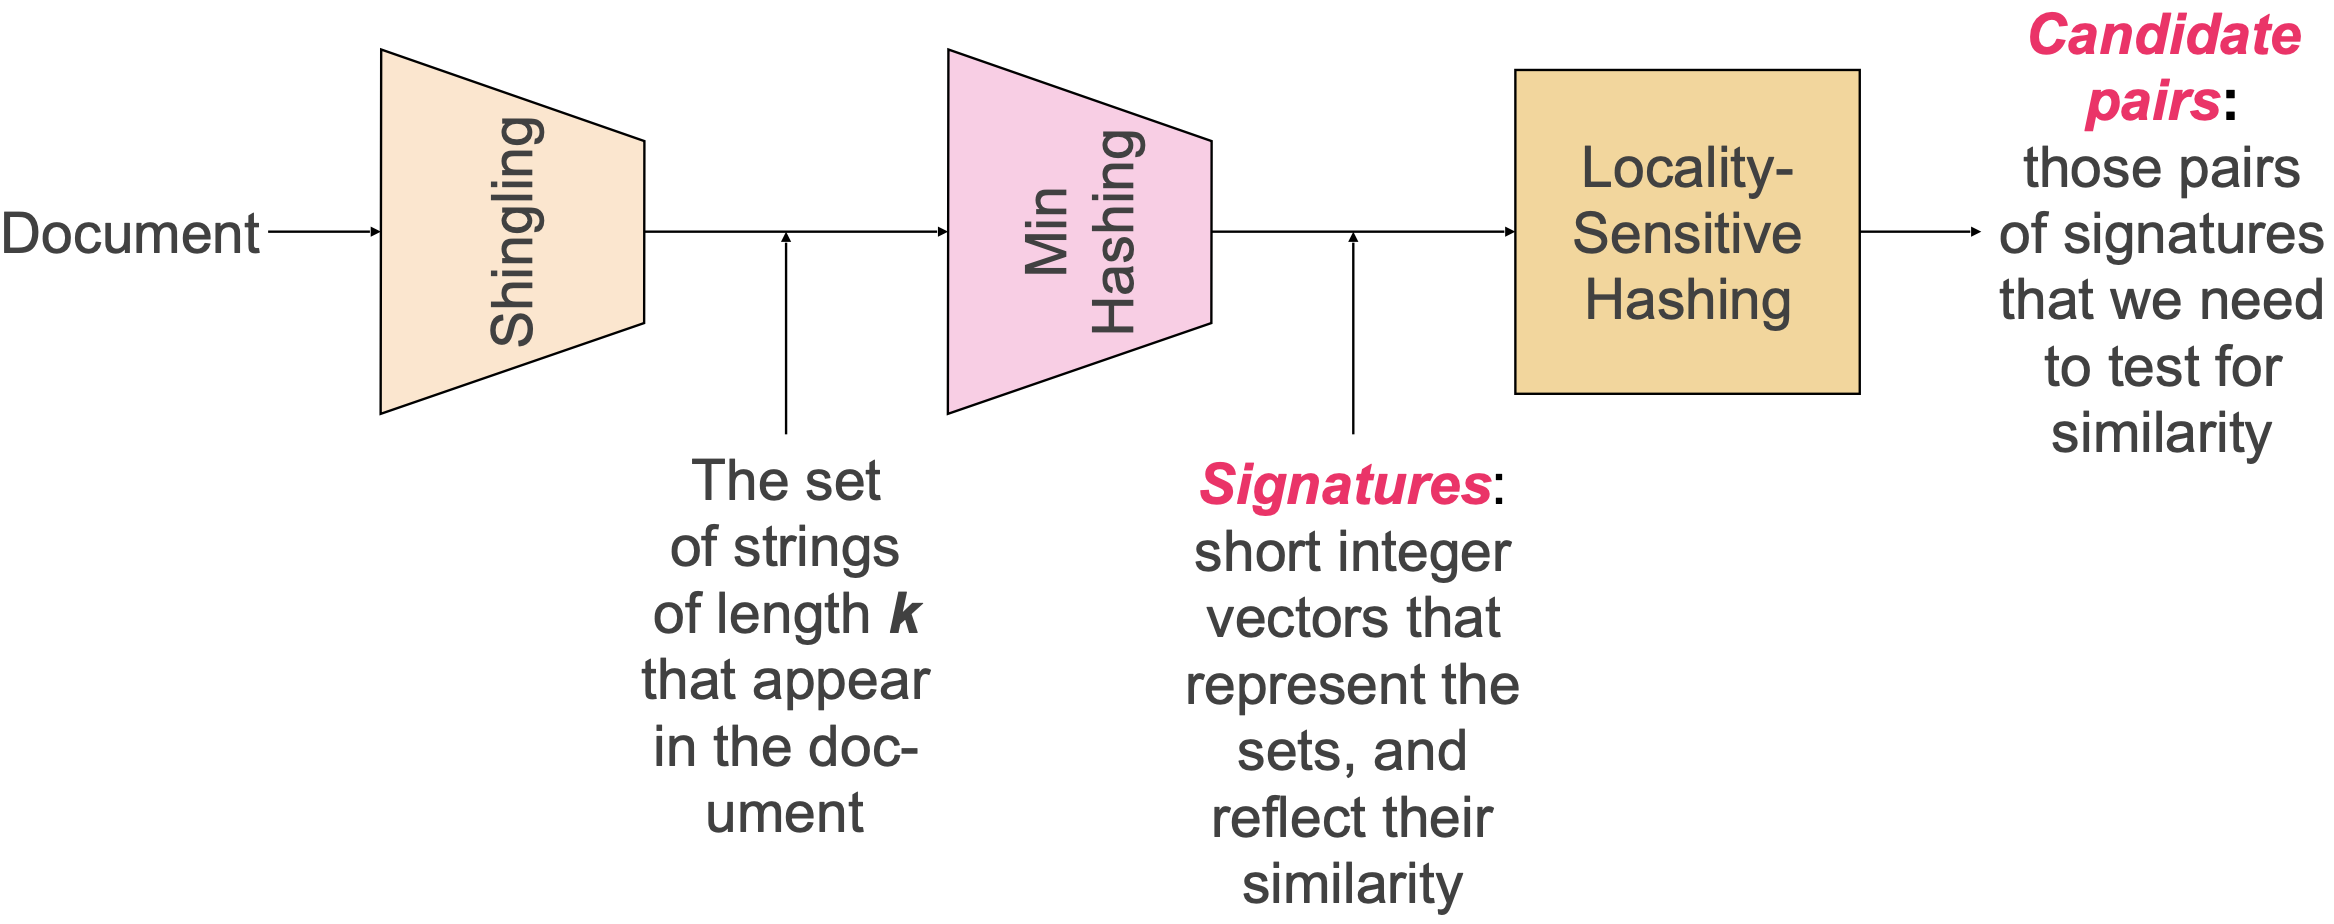
\includegraphics[scale=0.35]{figures/lsh.png}
 \caption{Locality-Sensitive Hashing}
\end{figure}


\section{LSH Steps}
\begin{enumerate}
 \item Shingling: Convert documents into sets of shingles.
 \item Min-Hashing: Convert large sets of short signatures, while preserving similarity (i.e. Jaccard similarity).
 \item Locality-Sensitive Hashing: Focus on pairs of signatures likely to be from similar documents.
\end{enumerate}
\begin{itemize}
 \item This results in candidate pairs, which are likely candidates with a high probability of being similar to the input document.
\end{itemize}

\section{Shingling}
Shingling is the process of converting documents to sets. Some simple approaches are to transform the document into sets of unique words, or "important" words.
The main problem is that the ordering of words has to be taken into account:

\subsection{Shingles}
A $k$-shingle (or $k$-gram) for a document is a sequence of $k$ tokens that appears in the document.
\begin{itemize}
 \item Tokens can be characters, words, or something else, depending on the application.
\end{itemize}

A modification of the $k$-shingle is to use shingles as a bag (multiset), and therefore counting equal sequences multiple times instead of only one.

\subsubsection{Similarity Metric for Shingles}
\begin{itemize}
 \item Document $D_i$ is a set of its $k$-shingles $C_i = S(D_i)$
 \item In this setting, each unique shingle is a dimension.
 \item The vectors will be very sparse as most documents does not contain most of the shingles.
\end{itemize}

A natural similarity measure is the \textbf{Jaccard Similarity}:

\begin{equation}
 sim(D_1, D_2) = \frac{\abs{C_1 \cap C_2}}{\abs{C_1 \cup C_2}}
\end{equation}

\subsubsection{Working Assumptions}
\begin{itemize}
 \item Documents that have lots of shingles in common have similar text, even if the text appears in different orders.
 \item $k = 5$ is ok for short documents.
 \item $k = 10$ is better for long documents.
\end{itemize}

\section{Min-Hashing}
Using pairwise Jaccard similarity directly to find near-duplicate documents would result in operations too complex and time consuming to handle. This is why min-hashing is used.

Min-hashing provides signatures (short integer vectors) that represent the sets and their similarity.

\subsubsection{Encoding Sets as Bit Vectors}
Many similarity problems can be formalized as:

Finding subsets that have a significant intersection.

\bigskip

This can be done efficiently by encoding sets using boolean vectors.

\bigskip
\begin{figure}[H]
 \centering
 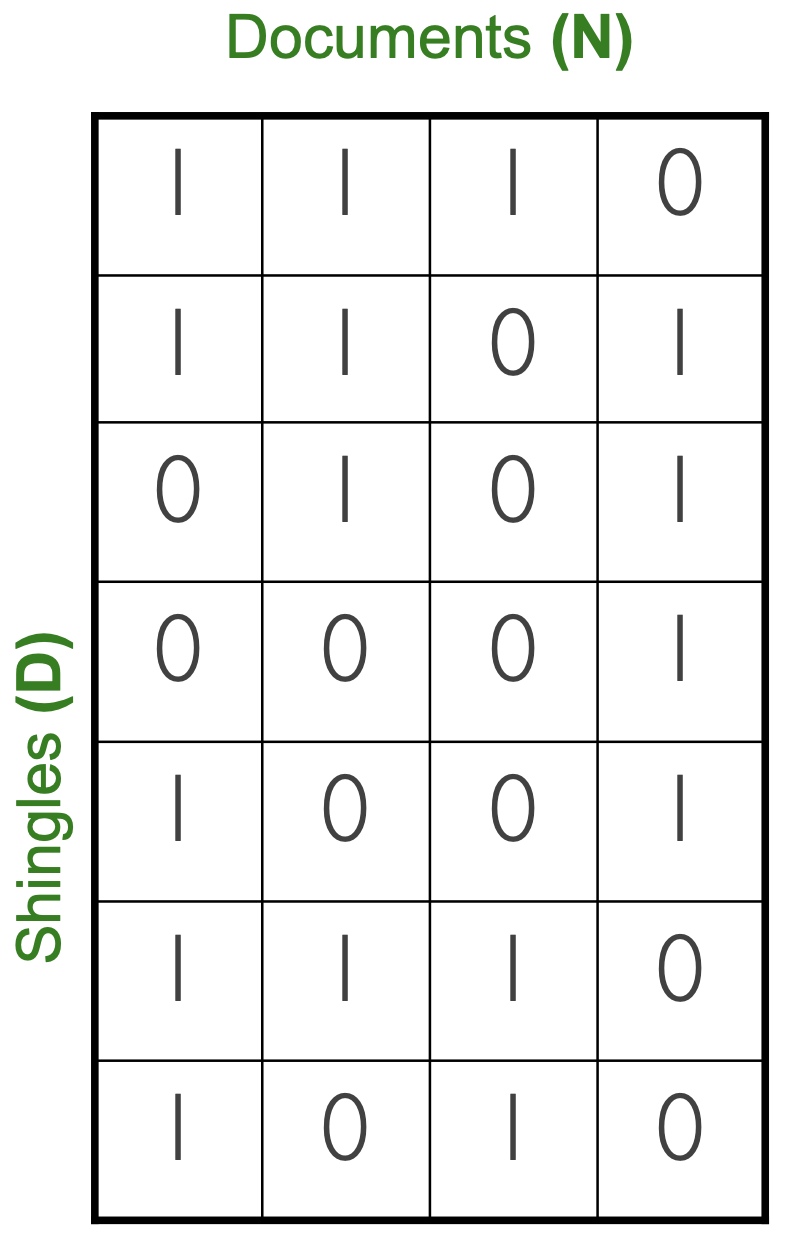
\includegraphics[scale=0.3]{figures/boolmatrix.png}

 \textit{Note:} $d(C_1, C_2) = 1 - \frac{\abs{C_1 \cap C_2}}{\abs{C_1 \cup C_2}} = 1 - \frac{3}{6}$
 \caption{Boolean Matrix}
\end{figure}

\subsection{Hashing Columns}
The key idea of hashing is to hash each column $C$ to a small signature $h(C)$ so that:
\begin{itemize}
 \item $h(C)$ is small enough to fit in the RAM.
 \item The Jaccard similarity is preserved.
\end{itemize}

The goal is to find a hash function so that if $sim(C_1, C_2)$ is high, there is a high probability that $h(C_1) = h(C_2)$, and vice versa.
The hash function places columns into a bucket, with the expected outcome being that most pairs of near-duplicate documents hash into the same bucket.

\bigskip

A suitable hash function for the Jaccard similarity is called \textbf{Min-Hashing}.

\subsection{Definition}
\begin{itemize}
 \item Imagine the rows of the boolean matrix permuted under random permutation $\pi$.
 \item Define a hash function $h_\pi(C)$ = the index of the first row in which column $C$ is $True$.
 \item Use several independent hash functions (that is, permutations) to create a signature of a column.
\end{itemize}

\begin{equation}
 \bm{h}_\pi\bm{(C)} = \bm{min}_\pi\pi\bm{(C)}
\end{equation}

Each unique combination of $1$s and $0$s can be classified as different types.

I.e. $A = 1, 1$, $B = 1, 0$, $C = 0, 1$, $D = 0, 0$.
If lower case letters denote the number of rows corresponding to the corresponding type, we get the following Jaccard similarity:
\begin{equation}
 sim(C_1, C_2) = \frac{a}{a+b+c}
\end{equation}
And the probability:
\begin{equation}
 Pr\left[h_\pi(C_1) = h_\pi(C_2)\right] = sim(C_1, C_2)
\end{equation}
And the thought-process is:

\begin{enumerate}
 \item Look down the columns $C_1$ and $C_2$ until the first $1$ appears.
 \item If the row is of type $A$, then $h(C_1) = h(C_2)$.
 \item If the row is of type $B$ or $C$, then $h(C_1) \neq h(C_2)$.
\end{enumerate}

\subsubsection{Similarity for Signatures}
\begin{itemize}
 \item The similarity of two signatures is the fraction of the hash functions in which they agree.
 \item Because of the Min-Hash property, the similarity of columns is the same as the expected similarity of their signatures.
\end{itemize}

\bigskip
\begin{figure}[H]
 \centering
 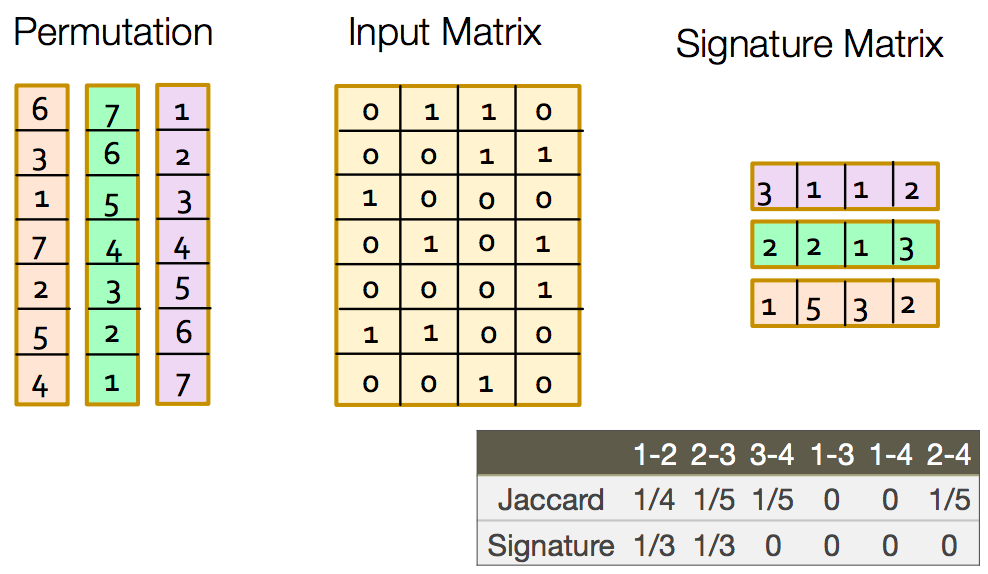
\includegraphics[scale=0.35]{figures/minhashing.png}
 \caption{Min-Hashing}
\end{figure}

\subsection{Process}
\begin{enumerate}
 \item Pick $k=100$ random permutations of the rows.
 \item Think of $\bm{sig(C)}$ as a column vector.
 \item $\bm{sig(C)[i]} = $ The index of the first row that has the value of $1$ in column $C$, given the $\bm{i}_{th}$ permutation.
 \item $\bm{sig(C)[i]} = \bm{min\left(\pi_i(C)\right)}$ 
\end{enumerate}

\section{LSH}
The goal of the locality-sensitive hashing process is to find documents with Jaccard similarity over some similarity threshold $s$.

The general idea is to use a function $f(x, y)$ that tells whether $x$ and $y$ is a candidate pair; a pair of elements whose similarity must be evaluated.

For Min-Hash matrices:
\begin{itemize}
 \item Hash columns of the signature matrix $M$ into many buckets,
 \item Each pair of documents that hashes into the same bucket is a candidate pair.
\end{itemize}

Columns $x$ and $y$ of $M$ are a candidate pair if their signatures agree on at leas the fraction $s$ of their rows.
$\bm{M}(i, x) = \bm{M}(i, y)$ for at least the fraction $s$ of $i$. It is expected that the documents $x$ and $y$ have the same Jaccard similarity as their signatures.

\bigskip

The main idea of LSH for Min-hashing is to hash columns of the signature matrix $M$ several times.
Then, arrange the columns so that only similar columns are likely to hash to the same bucket, with a high probability.
Finally, the candidate pairs are those columns that hash to the same bucket.

\subsection{Process of LSH}
\begin{enumerate}
 \item Divide matrix $M$ into $b$ bands of $r$ rows.
 \item For each band, hash its portion of each column to a hash table with $k$ buckets, while making $k$ as large as possible.
 \item The candidate column pairs are those bands that hash to the same bucket for more than one band.
 \item Tune $b$ and $r$ to catch most similar pairs, and minimize the number of non-similar pairs.
\end{enumerate}

\subsubsection{Simplified Assumptions}
\begin{itemize}
 \item There are enough buckets that columns are unlikely to hash to the same bucket unless they are identical in a particular band.
 \item It is assumed that all bands in the bucket are identical.
 \item These assumptions are only needed to simplify the analysis, not for the correctness of the algorithm.
\end{itemize}

\subsubsection{Some Probabilities}
Given the columns $C_1$ and $C_2$ with the similarity $s$, and that $b$ bands with $r$ rows is selected:
\begin{itemize}
 \item The probability that all rows in the band are equal $ = s^r$
 \item The probability that some rows in the band are unequal $ = 1 - s^r$
 \item The probability that no bands are identical after $b$ bands $ = (1-s^r)^b$
 \item The probability that at least one band is identical after $b$ bands $ = 1 - (1-s^r)^b$
\end{itemize}

\subsection{LSH Decisions}
Some parameters have to be adjusted to balance the false positives and negatives and get the most desired result when using LSH. This includes:
\begin{itemize}
 \item The number of Min-Hashes (rows of $M$).
 \item The number of bands $b$.
 \item The number of rows $r$ per band.
\end{itemize}

\subsection{Summary}
\begin{itemize}
 \item Tune $M$, $b$, and $r$ to get almost all pairs with similar signatures, but eliminate most pairs that do not have similar signatures.
 \item Check in the main memory that candidate pairs do have similar signatures.
 \item Optional: In another pass through the data, check that the remaining candidate pairs represent similar documents.
\end{itemize}
